\documentclass[12pt]{article}
\usepackage{amsmath}
\usepackage[top=1in, bottom=1in, left=0.8in, right=1in]{geometry}
\usepackage{multicol}
\usepackage{wrapfig}
\usepackage{listings}
\usepackage{enumitem}
\usepackage{comment}
\usepackage{tikz}
\usepackage{hyperref}
\usepackage{caption}
\usepackage{subcaption}
\usepackage[ruled,vlined]{algorithm2e}
\lstset{language=Java, basicstyle={\small\ttfamily}, columns=flexible, belowskip=0mm}
\setlength{\columnsep}{0.1pc}

\begin{document}

\noindent
CS 440: Intro to Artificial Intelligence \hfill Assignment 1\newline
Fall 2022 \hfill Due October 19, 2022, 11:59 p.m.

\noindent
\rule{\linewidth}{0.4pt}

\vspace{.5cm}

\textbf{Names}: Will Chen, Noel Declaro, Afsana Rahman

\vspace{.5cm}

\textbf{Overview}:  This document contains answers to all questions, Problems 1-5, in Assignment 1. Instructions on how to run our program for Problem 1 are detailed in the \texttt{README.txt} file. The source code for this file should also be in the zip folder. 

\noindent
\rule{\linewidth}{0.4pt}

\vspace{.5cm}

\textbf{Problem 1 (65 points):}

\begin{enumerate}[label=(\alph*)]

  %%% Question (a)
  
  \item \textbf{Creating and visualizing grids.} (10 points) The \texttt{interface.py} script runs the implemented algorithms and displays the results. The input field at the top of the display allows for the user to set an S-vertex and a possible input to display calculated F, G, and H values into the terminal. Within the interface script there are commands that allow the user to load any grid and select either the A* or Theta* algorithm to run. A more detailed description of using the interface is in the \texttt{README.txt} file of the submitted code. The expected visual output of a small sample grid is shown in  Figure 1.

  \begin{figure}[h]
    \centering
    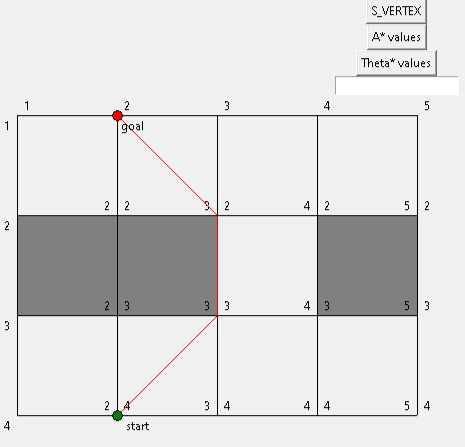
\includegraphics[scale=0.85]{homework1/images/testingscreenshots/interface.jpg}
	\caption{Example visual using the 4x3 grid in the assignment writeup.}
	\label{fig:fig1}
  \end{figure}

  %%% Question (b)
  \item \textbf{Manually computing shortest paths.} (5 points) 

  \begin{figure}[h]
    \centering
    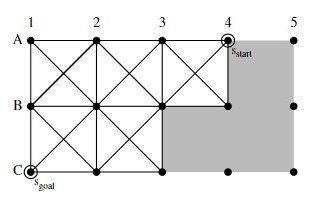
\includegraphics[scale=1.2]{homework1/images/probdescrips/figure7original.jpg}
	\caption{Example search problem - Figure 7 from Assignment 1A writeup.}
	\label{fig:fig2}
  \end{figure}

  \begin{enumerate}
  
      \item[(i)] \textbf{A* algorithm - shortest grid path.} In order to find the shortest path from the start vertex $s_{start} = (4,1)$ to the goal vertex $s_{goal} = (1,3)$, we must 1) compute the f-values of the valid adjacent vertices from the start point, 2) find the minimum of this set, and then 3) expand the vertex with the minimum cost and repeat the steps. In order to compute an f-value for a given vertex $(s^x, s^y)$, we sum its $g(s)$ value and $h(s)$ value, where $g(s)$ is equal to the current vertex's distance from $s_{start}$, and 
      \begin{equation}
          \scriptsize h(s) = \sqrt{2}\cdot\min(|s^x - s_{goal}^x|,|s^y - s_{goal}^y|) + \max(|s^x - s_{goal}^x|,|s^y - s_{goal}^y|) - \min(|s^x - s_{goal}^x|,|s^y - s_{goal}^y|)
      \end{equation}
      
      Using this algorithm, we retrieve the traces/computations shown in Figure 3. The red circles denote which vertex is being expanded, and the blue arrows denote potential vertices to expand (captioned with their respective f-values written as the sum of their g- and h-values). The red dotted line shown in Figure 3(d) shows the final shortest path (from $s_{start}$ to $s_{goal}$) found by tracing back through the vertices previously expanded.
      \begin{figure}
          \begin{subfigure}{0.5\textwidth}
            \centering
            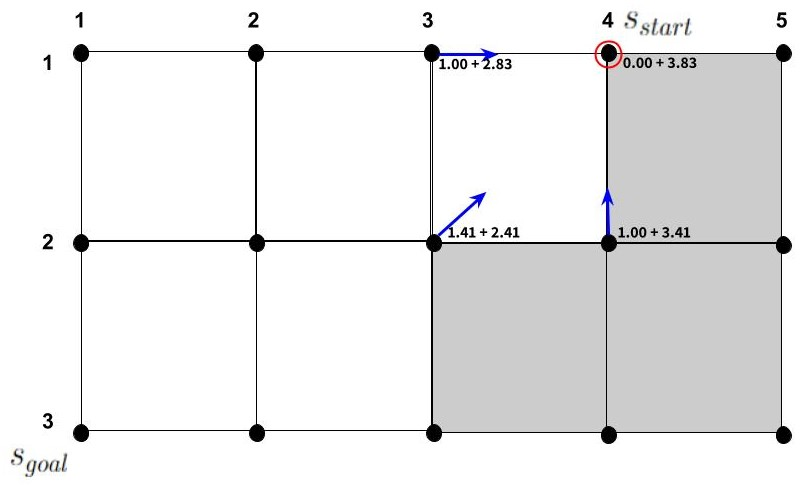
\includegraphics[width=\textwidth]{homework1/images/drawndiagrams/prob1bi/figure2a.jpg}
            \caption{}
            \label{fig:fig2a}
          \end{subfigure}
          \begin{subfigure}{0.5\textwidth}
            \centering
            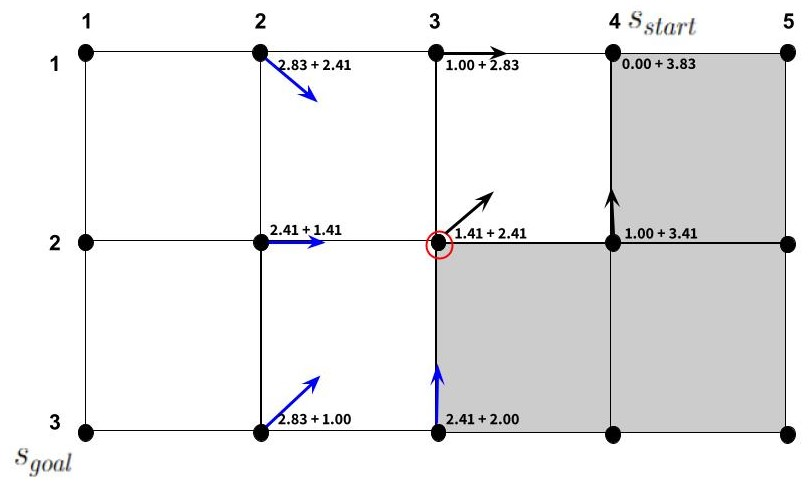
\includegraphics[width=\textwidth]{homework1/images/drawndiagrams/prob1bi/figure2b.jpg}
            \caption{}
            \label{fig:fig2b}
          \end{subfigure}
          \begin{subfigure}{0.5\textwidth}
            \centering
            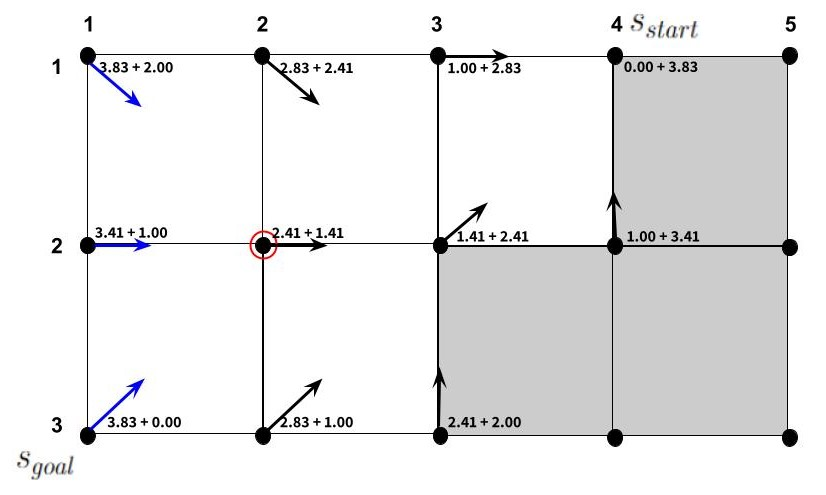
\includegraphics[width=\textwidth]{homework1/images/drawndiagrams/prob1bi/figure2c.jpg}
            \caption{}
            \label{fig:fig2c}
          \end{subfigure}
          \begin{subfigure}{0.5\textwidth}
            \centering
            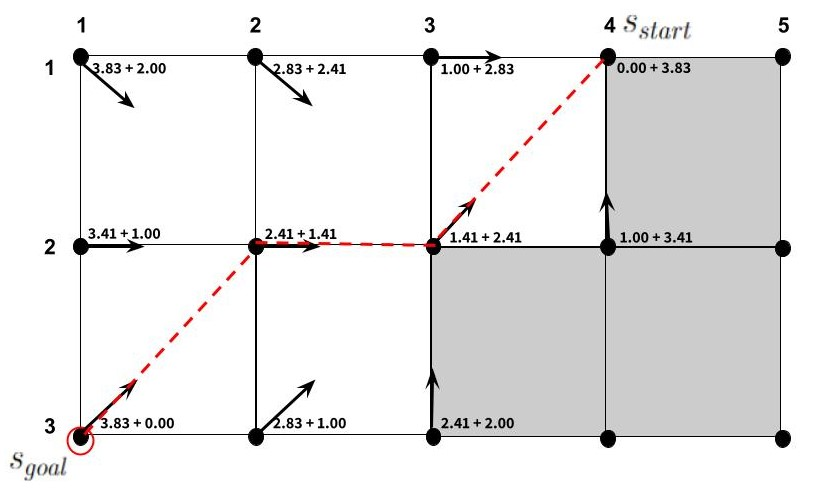
\includegraphics[width=\textwidth]{homework1/images/drawndiagrams/prob1bi/figure2d.jpg}
            \caption{}
            \label{fig:fig2d}
          \end{subfigure}
          \caption{Trace of A* Algorithm}
      \end{figure}

      \item[(ii)] \textbf{Theta* algorithm - shortest any-angle path.} In order to find the shortest any-angle path from the same start and goal points as the previous part, we will conduct a similar search/use a similar algorithm with some slight adjustments. Now, our $g(s)$ values will be computed as the cost from the start \textit{directly} to the given point, and the $h(s)$ values will be computed as the estimated cost from the given point directly to the goal.
      
      Using this algorithm, we retrieve the traces/computations shown in Figure 4. The red circles denote which vertex is being expanded, and the blue arrows denote potential vertices to expand (captioned with their respective f-values written as the sum of their g- and h-values). The red dotted line shown in Figure 4(d) shows the final shortest path (from $s_{start}$ to $s_{goal}$) found by tracing back through the vertices previously expanded.
      \begin{figure}
          \begin{subfigure}{0.5\textwidth}
            \centering
            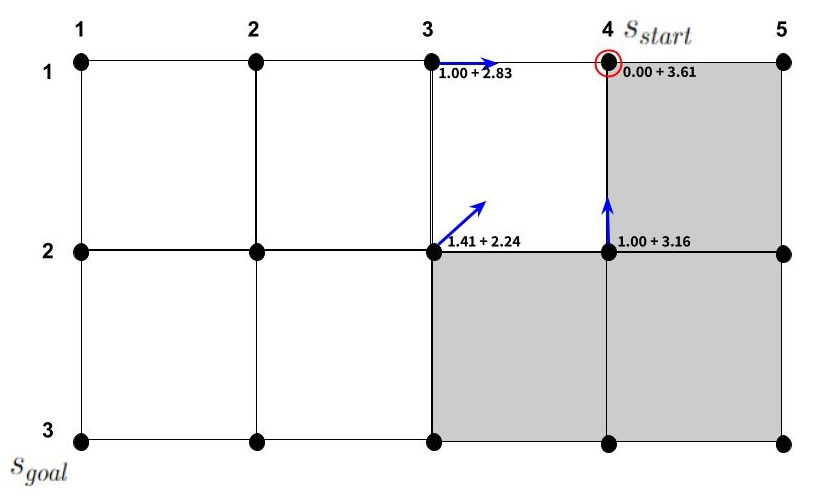
\includegraphics[width=\textwidth]{homework1/images/drawndiagrams/prob1bii/figure3a.jpg}
            \caption{}
            \label{fig:fig3a}
          \end{subfigure}
          \begin{subfigure}{0.5\textwidth}
            \centering
            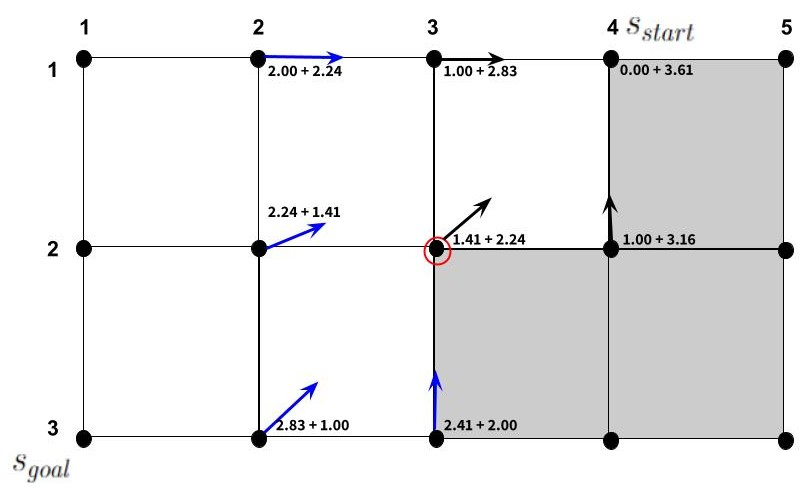
\includegraphics[width=\textwidth]{homework1/images/drawndiagrams/prob1bii/figure3b.jpg}
            \caption{}
            \label{fig:fig3b}
          \end{subfigure}
          \begin{subfigure}{0.5\textwidth}
            \centering
            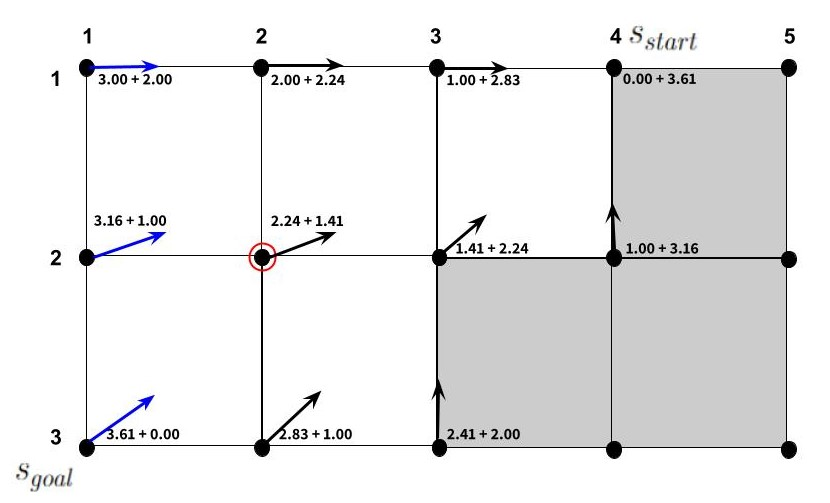
\includegraphics[width=\textwidth]{homework1/images/drawndiagrams/prob1bii/figure3c.jpg}
            \caption{}
            \label{fig:fig3c}
          \end{subfigure}
          \begin{subfigure}{0.5\textwidth}
            \centering
            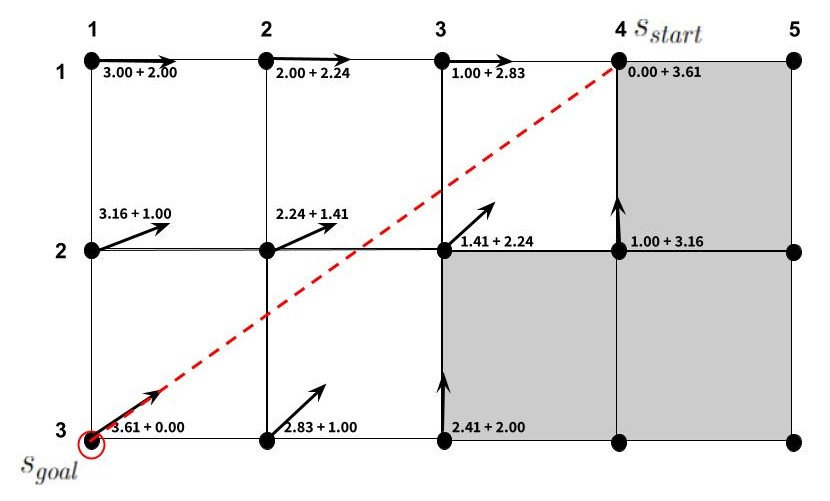
\includegraphics[width=\textwidth]{homework1/images/drawndiagrams/prob1bii/figure3d.jpg}
            \caption{}
            \label{fig:fig3d}
          \end{subfigure}
          \caption{Trace of Theta* Algorithm}
      \end{figure}
      
  \end{enumerate}
  

  %%% Question (c)
  \item \textbf{A* algorithm implementation.} (5 points) Implementation of A*. If a vertex has been expanded, it is added to the \textbf{closed list}. This particular list is a Hashmap so that confirming whether or not a node is in the list is an $O(1)$ operation on average. The key is its vertex in string representation, and its value is a \textbf{HeapNode}. 
  
  \textbf{HeapNode} is a class object created to store necessary information on a node. It contains representations of the vertex in an integer array, string, and integers. The string of its parent, $g(n)$ the true distance to start, and $f(n)$ the heuristic and true distance sum. This information can all be called in $O(1)$ time. 
  
  The \textbf{open list} of potential expansion is a minimum binary heap, using a \textbf{MinHeap} implementation described in 1(f). Deciding whether or not a vertex is valid (in the grid) or can be added (already added to the open list or closed list) is determined by a 2D array \textbf{already expanded} keeping track of vertices added to the open list, and does not allow a re-visitation. This is a space addition of $O(n)$ equivalent to the size of the grid.  
  
  The file is read in using a Scanner. A second 2D array of blocked \textbf{cells} is maintained that reads in each blocked cell and marks it with $O(n)$ space equivalent to the size of the grid. 

  A function, \textbf{checkPaths()} indicates whether or not an adjacent vertex can be added to the open list, by checking whether or not the vertex is in the bounds of the map, if it is in a closed list, or if it has already been put into the open list. It then sends the possible nodes to be added to the open list as nodes.
  
  Nodes are popped from the open list in priority order as the act of expansion as they are added to the closed list. This continues until there are no nodes left in the open list or the node popped is matched to the goal. If no nodes are left that implies no path, and a file is output stating such, otherwise once the goal node is found, the vertices are printed to an output file in reverse order, from goal to start by following the chain of parent strings and checking the closed list to go back up the order. 

  
  %%% Question (d)
  \item \textbf{Theta* algorithm implementation.} (10 points) The base above structure for A* in 1C is exactly the same as Theta. The key difference is that the in \textbf{LineOfSight()} function is added, which allows nodes to change their parent node if a better node is available to create a shorter path. \textbf{UpdateVertex()} is called each time a node is being added to the open list, and it is where the LineOfSight function is called to determine parentage. Essentially, each additional node adds the surrounding adjacent unchecked vertices to be put into the open list. Prior to insertion, the nodes are checked against their grandparent (parent of the parent node) to see if there is a straight line between them through LineOfSight. If there is a straight line, and it is shorter than through the parent to the child, then the triangle inequality holds, and the child’s parent is set to the grandparent, making the adjustments in the child’s $g(n)$ function. If LineOfSight is false, then there is no better existing parent, which means the parent child relationship remains the standard as in A*. 
  
  The LineOfSight function is relatively cheap, based on the distance between the grandparent and child node. Since the maximum time run is a multiple function of the hypotenuse between the diagonal corners of a grid or $O(\sqrt{r^2 + c^2})$ for rows r and columns c.  However, it is generally on a much smaller order based on the straight line distance between the two points. 
  
  Due to the nature of adding nodes one at a time, this eventually creates long straight line distances from start to intermediate vertices, and allows freedom of all angle and parent distance traversal, as prior parents in A* were required to be adjacent to the child vertex. 
  
  The\textbf{ already expanded} 2D array used in A* was set up as to not allow any repeated additions to the open list, however this array serves a slightly different purpose in Theta. As re-visitation is allowed in order to determine whether or not the parent of a child node is the parent or grandparent, the main role of the already expanded array in Theta* is to detect if a vertex is already in the open list, which would indicate that there are already $f(n)$, $g(n)$, and $h(n)$ values for the node. These values are checked using the triangle inequality for consistency. If a node is not in the open list already, these values are defaulted to maximums so they can be assigned through the UpdateVertex function.
  
  Both A* and Theta outputs the pathing tree in goal to start order to a new file in the form x,y. If there is no valid route, then a file is created stating there is no valid path.


  %%% Question (e)  
  \item \textbf{Proof regarding A* algorithm.} (5 points) In order to prove that our A* algorithm will always find the shortest path -- or, in other words, to prove that our A* algorithm is optimal -- we need to prove that our heuristic $h(s)$ is consistent (theorem provided in class). As defined in class, a heuristic is considered consistent if 
  \begin{equation}
      \forall(s, a, s'): h(s) \leq c(s, a, s') + h(s')
  \end{equation}
  where $c(s, a, s')$ is the step cost for going from $s$ to $s'$ using action $a$. In plain English terms, this means that for every step taken throughout our A* algorithm, the estimated cost of the current point to the goal ($h(s)$) should always be less than or equal to the sum of the cost to get to the next point from the current point ($c(s, a, s')$) and the cost from the next point to the goal ($h(s')$). For the sake of easier reading/convenience, here is $h(s)$ (Equation 1) re-written, where $\Delta s^x = s^x - s_{goal}^x$ and $\Delta s^y = s^y - s_{goal}^y$:
  \begin{equation}
      h(s) = \sqrt{2}\cdot\min(|\Delta s^x|, |\Delta s^y|) + \max(|\Delta s^x|, |\Delta s^y|) - \min(|\Delta s^x|, |\Delta s^y|)
  \end{equation}
  The heuristic essentially estimates the maximal diagonal distance that can possibly be taken to get to the goal given the constraints of the grid, and then adds the leftover necessary up/down/left/right steps after going as many diagonals as possible. To explain further: $\sqrt{2}\cdot\min(|\Delta s^x|, |\Delta s^y|)$ gives us the maximum possible of diagonals we can travel (as to avoid going horizontally or vertically), and then we add the steps leftover that are required to get to the goal ($\max(|\Delta s^x|, |\Delta s^y|)$) while compensating for the diagonal distance taken ($- \min(|\Delta s^x|, |\Delta s^y|)$). If there is a straight strictly horizontal or strictly vertical path to the goal from the current point, then $\sqrt{2}\cdot\min(|\Delta s^x|, |\Delta s^y|) = 0$ and $h(s) = \max(|\Delta s^x|, |\Delta s^y|)$.  This logic ensures that the heuristic provides the shortest estimated path distance from any given point $(s^x, s^y)$. 
  
  In order to prove that the heuristic is consistent (Equation 2), we only need to ensure that the estimated distance from the current point is less than or equal to the sum of the cost of the next step and the distance from the next point to the goal. There are really only two things that can happen at this stage: either we move diagonally towards the goal (optimal), or we move up/down/left/right due to being unable to move diagonally. Inability to move diagonally can be due to two reasons: either there is a straight horizontal or vertical grid path to the goal (so we remain equal to our original estimated distance from the previous point), or a diagonal is blocked by a blocked cell in the grid, meaning we must move around it (taking up much more distance than previously estimated). In the case of finding the goal point and its $h(s)$ value, both $\max(|\Delta s^x|, |\Delta s^y|)$ and $\min(|\Delta s^x|, |\Delta s^y|)$ will be 0, meaning $h(s_{goal})$ will always be 0. In any case as just described, the estimated $h(s)$ value at a given point will always be less than or equal to the estimated $h(s')$ value at the next point, meaning that the heuristic is consistent and this A* algorithm is optimal.
  
  %%% Question (f)
  \item \textbf{Extra credit: Using binary heaps.} (10 points) We have implemented a binary heap as a Minimum Heap, holding information about its capacity, size, and an array of nodes that stores information on vertices. This acts as a priority queue based on the minimum possible $g(n) + h(n)$ value of each vertex.
  
  The binary heap is able to pop the root node, as well as remove a given node if it exists within the heap. The \textbf{popMin()} function must call a function \textbf{heapify()} that preserves min-heap order of the nodes when a node is removed, shifting nodes through the heap based on the number of layers in the tree, representing an $O(logn)$ time complexity. 
  
  The \textbf{insert()} function also represents an $O(logn)$ time complexity for each node, as the worst case is a node must be sent all the way up a tree when being inserted. 
  
  The \textbf{remove()} function occurs in $O(n)$ time, as it is required to iterate through all nodes to determine if the search target exists. 
  
  Helper methods are added to either get child left and right indices or nodes, as well as parent indices and nodes. \textbf{isEmpty()} and \textbf{peek()} are also included, and these are constant time methods. A \textbf{print()} function is also included that prints nodes in tree order and describes the children of the tree. 
  
  A \textbf{resize()} function is used to increase the size of the array allocation if insertions exceed capacity of the node array. It doubles the allocated array space, and is an $O(n)$ task as it must iterate through all nodes of the initial array to insert them into the new array for increased capacity.

  %%% Question (g)
  \item \textbf{Optimizing A* and Theta* implementations.} (5 points) As we did not have either algorithm implemented in our first submission, we cannot make a comparison to this current one. However, the optimization/time complexity/space complexity regarding our current implementations are described in the previous questions.

  %%% Question (h)
  \item \textbf{Comparing heuristics to run times.} (10 points) The grids used are with the ‘grids’ folder in the provided code. Each of the grids can be displayed using the interface. The grids for all experiments follow the condition that they are size of 100 x 50 with 10\% chance of being blocked. Through running experiments, we obtained the average run times of each algorithm over 50 grids, shown in Figure 5.

  Some other observations include:
    \begin{itemize}
        \item Theta* requires less tracing compared to A*. The is most apparent when looking at the \texttt{test\_solution.txt} files when the grids are loaded and the algorithm is ran. A* will require more lines to trace out the plots of solutions while Theta* uses much less lines. Since Theta* has a larger fringe to explore, more optimal paths are available to Theta*.
        \item To test this experiment the same process is used with the 50 grids but it counts the numbers of vertices in the solution tracing after each run. At the end it then averages them. 
    \end{itemize}

    \begin{figure}
        \begin{subfigure}{\textwidth}
            \centering
            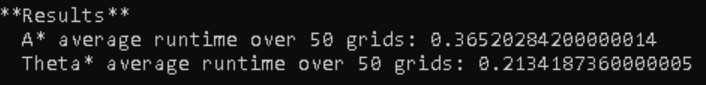
\includegraphics[scale = 0.7]{homework1/images/testingscreenshots/prob1ha.jpg}
            \caption{}
            \label{fig:prob1ha}
        \end{subfigure}
        \begin{subfigure}{\textwidth}
            \centering
            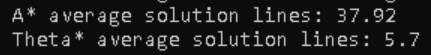
\includegraphics[scale = 0.8]{homework1/images/testingscreenshots/prob1hb.jpg}
            \caption{}
            \label{fig:prob1hb}
        \end{subfigure}
        \caption{Results from running experiments on sample 100x50 grids.}
    \end{figure}


  %%% Question (i)
  \item \textbf{Appropriate h-values for A* and Theta*.} (5 points) It is appropriate to have different heuristic functions for these A* and Theta* algorithms. The A* algorithm is limited to grid lines/diagonals within cells, so its heuristic function appropriately corresponds to maximizing the diagonals that can be taken, along with the minimum horizontal/vertical distance needed after that. In other words, since the A* algorithm is under more constraint, a more constrained/accurate heuristic is appropriate here. In contrast, the Theta* algorithm is more free to take shortcuts between nonadjacent cells, so it should be more liberal in its estimations (using a heuristic that computes \textit{direct} cost between two vertices).

  %%% Question (j)
  \item \textbf{Cases where minimal path was not found.} (5 points) Theta* does not provide an optimal path due to the nature of the line of sight checking algorithm and the determination of parentage of a child node. The child node either chooses the grandparent if it is in line of sight, or the parent if it is not. Two examples of differences in shortest path are shown in Figure 6; each example grid shows the shortest path found by A* (blue line), found by Theta* (red line), and the true shortest path computed by hand (green line). Computations of path lengths are given in the figure caption.

    \begin{figure}
        \begin{subfigure}{0.47\textwidth}
            \centering
            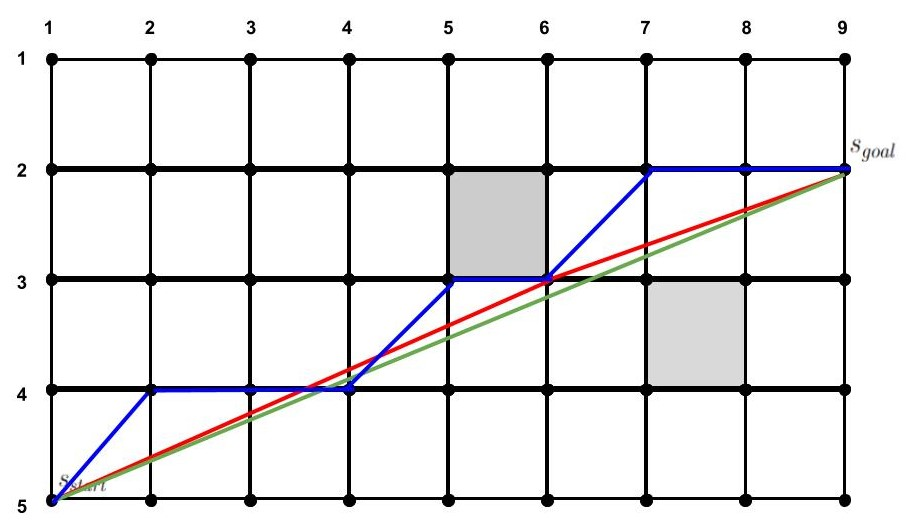
\includegraphics[width=\textwidth]{homework1/images/drawndiagrams/prob1j/prob1ja.jpg}
            \label{fig:prob1ja}
        \end{subfigure}
        \begin{subfigure}{0.46\textwidth}
            \centering
            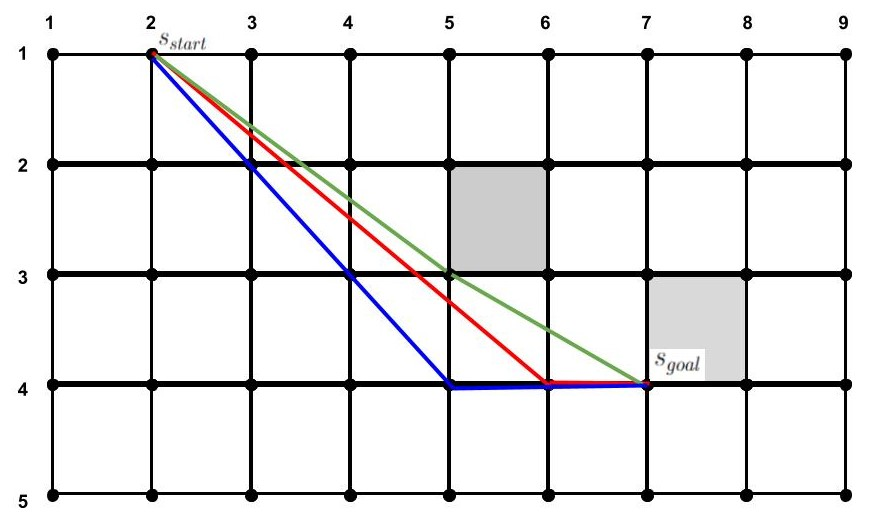
\includegraphics[width=\textwidth]{homework1/images/drawndiagrams/prob1j/prob1jb.jpg}
            \label{fig:prob1jb}
        \end{subfigure}
        \caption{Shortest paths computed by A* algorithm, Theta* algorithm, and the true shortest path computed by hand. In the grid in (a), the A* algorithm provides a path length of roughly 9.243, Theta* provides a path length of 8.547, and the true shortest path has length 8.544. In the grid in (b), the A* algorithm provides a path length of roughly 6.243, Theta* provides a path length of 6.000, and the true shortest path has length 5.842.}
    \end{figure}

  %%% Question (k)
  \item \textbf{Extra credit: Using visibility graphs.} (10 points) This was not implemented.

  %%% Question (l)
  \item \textbf{Theta* expanded vertices decreasing in f-values.} (5 points) An example grid where the f-values of Theta* may be decreasing but the h-values remain consistent is a grid where the shortest path found is not a path along the grid lines (in other words, a path with some shortcut where the g-value of some vertex does not follow the exact grid path of the previously selected vertices -- a found shortcut). This is the case in both the example trace of Theta* in the assignment write-up, and the Theta* trace in 1(b). In both cases, the h-values are consistent -- Theta* computes the h-value as the direct cost/shortest distance, so it cannot be overestimated unless choosing to expand on a vertex further from the goal -- but the f-value of the goal vertex is smaller than the f-value of the vertex before it. Another example is provided in Figure 7.

    \begin{figure}
        \begin{subfigure}{0.5\textwidth}
            \centering
            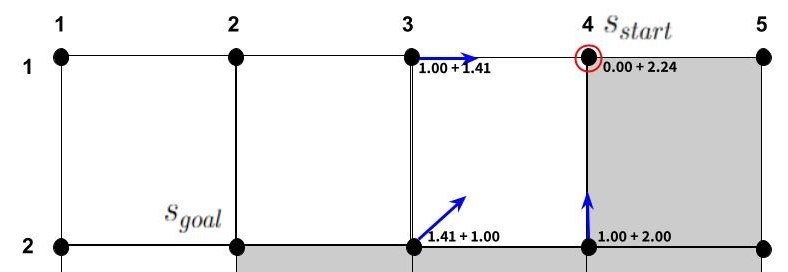
\includegraphics[width=\textwidth]{homework1/images/drawndiagrams/prob1l/prob1la.jpg}
            \caption{}
            \label{fig:prob1la}
        \end{subfigure}
        \begin{subfigure}{0.5\textwidth}
            \centering
            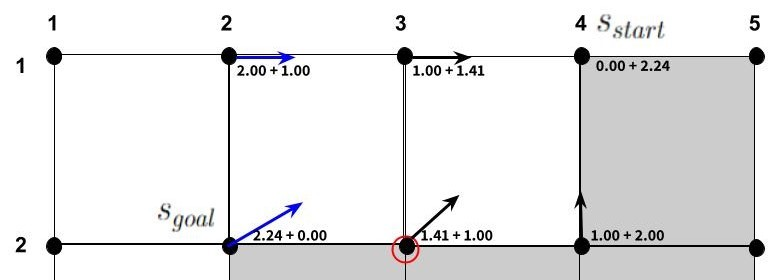
\includegraphics[width=\textwidth]{homework1/images/drawndiagrams/prob1l/prob1lb.jpg}
            \caption{}
            \label{fig:prob1lb}
        \end{subfigure}
        \begin{subfigure}{\textwidth}
            \centering
            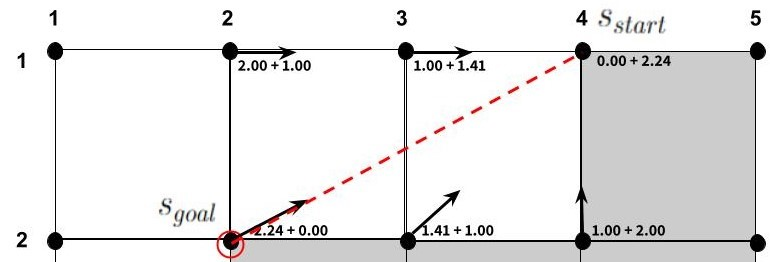
\includegraphics[scale = 0.7]{homework1/images/drawndiagrams/prob1l/prob1lc.jpg}
            \caption{}
            \label{fig:prob1lc}
        \end{subfigure}
        \caption{Example trace of Theta* with decreasing f-values ((3,2) $\xrightarrow{}$ (2,2))}
    \end{figure}

\end{enumerate}

\pagebreak

\rule{\linewidth}{0.4pt}
\vspace{.2cm}

%%%%%%%%%%%%%%%%%%%%%%%%%
%%%%%%%%%%%%%%% Problem 2
%%%%%%%%%%%%%%%%%%%%%%%%%
\textbf{Problem 2 - Adversarial Search (10 points):}

\begin{figure}[h]
    \centering
    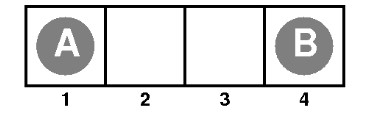
\includegraphics{homework1/images/probdescrips/prob2.jpg}
	\caption{Start position of a simple game.}
	\label{fig:prob2}
\end{figure}

\begin{enumerate}[label=(\alph*)]
    \item \textbf{Complete game tree.} The complete game tree is shown in Figure 9(a). Each game state is written as $(s_A, s_B)$, where $s_A$ and $s_B$ denote their respective token locations according to the game board in Figure 8. Terminal states are singly-boxed with its game value in the circle next to it. Loop states are doubly-boxed with its game value labeled with ``?".

    \item \textbf{Minimax algorithm.} The revised game tree with minimax values is shown in Figure 9(b). Loop states kept their ``?" values. When conducting the minimax algorithm to obtain values for the rest of the tree, a definite value is defaulted as a better choice over a ``?" (we consider ending the game as more optimal than a loop state); if there is no other option, then the parent state takes on the ``?" value as well. 

    \item \textbf{Why minimax algorithm fails.} The standard minimax algorithm fails with this particular game because the game reaches loop states where the search tree could potentially branch on infinitely. This poses a problem if we use the DFS algorithm to explore the game tree; the algorithm would iterate infinitely. 
    
    In order to fix this issue in the algorithm, we can implement some form of pruning; we can implement an evaluation function to determine usefulness of states, and/or a cutoff check that is free to cut off a search at a certain depth so the tree does not iterate states infinitely. A possible cutoff/evaluation of a state for this particular game could check whether the state has been repeated from the moves already made, and cut off search there (as shown in the tree for part (b)). Like before, loop states are considered as a sub-optimal move compared to true terminal states.

    This particular strategy is not useful/optimal for games that have an element of chance, games that have some variation in scoring, or games that may result in draws.  Specifically for games that may end in ties, it's difficult to discern how a ``?" state actually compares to a drawn state; in this specific example, the positions (1,4) and (2,4) are considered loop states further down the tree, but if the optimal path is taken from these particular leaves, it results in a win for player A (meaning a ``?"/loop state is not always necessarily a draw). 

    \begin{figure}
        \begin{subfigure}{0.5\textwidth}
            \centering
            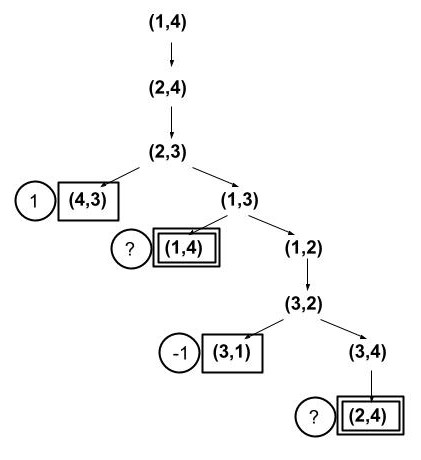
\includegraphics[scale=0.7]{homework1/images/drawndiagrams/prob2a.jpg}
            \caption{}
            \label{fig:prob2a}
        \end{subfigure}
        \begin{subfigure}{0.5\textwidth}
            \centering
            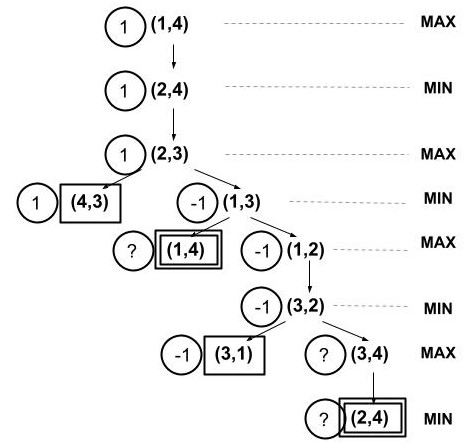
\includegraphics[width=\textwidth]{homework1/images/drawndiagrams/prob2b.jpg}
            \caption{}
            \label{fig:prob2b}
        \end{subfigure}
        \caption{Complete game trees.}
    \end{figure}

    \item \textbf{Proof regarding game size.} The 4-square game can be generalized to $n$ squares for any $n > 2$. Assuming the most optimal path is taken for each piece in any game, we can prove using induction that A will always win when $n$ is even and B will always win when $n$ is odd. 

    The base case for B winning would be when $n = 3$, where A must step forward and B is able to hop over it to its winning position. The base case for A winning would be when $n = 4$; the winning/optimal path for A is shown in the game tree in the previous parts of this problem. When expanding the board by two spaces -- to board sizes $n = 5$ and $n = 6$, respectively -- the first move by each player results in the same sub-game shown in each respective base case. (For $n = 5$, one move from A and then one from B essentially results in the same board as the ``B wins" base case -- the same applies for $n = 6$, where the two moves essentially result in the $n = 4$ board, the ``A wins" base case.) This pattern continues for all boards with $n > 2$; an odd-numbered board will eventually shrink down to an $n = 3$ board situation, and an even-numbered board will eventually shrink down to an $n = 4$ situation. In general, for odd-numbered boards, B will reach its goal before A (hopping over A at the center like in its $n = 3$ board base case, thus making more progress than A towards the goal), and for even-numbered boards, A will reach its goal before B (A will hop over B first like in its $n = 4$ base case, making more progress).

    The only contingency is if the players do not play optimally/move backward at some point. If the player who is slated to win the game moves backward, then the other player simply can move forward and make more progress towards its goal than the other player. At that point, the originally-slated-to-win player has to make several more moves to compensate for the ground they lost by moving backwards, whereas the other player now has less space to their goal in comparison.
     
\end{enumerate}


\rule{\linewidth}{0.4pt}
\vspace{.2cm}

%%%%%%%%%%%%%%%%%%%%%%%%%
%%%%%%%%%%%%%%% Problem 3
%%%%%%%%%%%%%%%%%%%%%%%%%
\textbf{Problem 3 - Local Search (10 points):}
\begin{enumerate}[label=(\alph*)]
    \item \textbf{Hill-climbing without simulated annealing.} The random part of simulated annealing is not necessary when there exists only one global maximum -- one ``hill" -- and no local maxima or plateaux when mapping the value function.
    \item \textbf{Simulated annealing without hill-climbing.} Hill-climbing is not necessary when the value function's landscape has no true global maximum, or in other words, has no definite optimal state. In other words, there are no ``hills" in the value function graph; it is never clear when we are approaching a solution regardless.
    \item \textbf{When simulated annealing is useful.} Simulated annealing is most useful when there is a global maximum and there are some local maxima and/or plateaux. The random generation through simulated annealing is useful for not getting stuck in shoulders/returning local maxima without exploring the entire landscape, and instead finding the global maximum (optimal state) through its random generation. 
    \item \textbf{Simulated annealing improvements.} In simulated annealing, instead of storing only a few states at a time (staying entirely local, focusing on the current and next states), we could also keep track of which particular state had the highest value from throughout the search and return that value at the end, regardless of the current state at the end of the schedule.
    \item \textbf{Simulated annealing with more memory.} With the capability of storing 2 million states, it would prove useful to run simulated annealing on 1 million states, pick the best 1 million states out of the original 1 million states + the new 1 million states generated, and continue the process until the global maximum is found. For example, two different states can be chosen where (1) there appears to be a hill/local maximum and (2) the most optimal state found so far, so a search can be conducted on states between those two points. This could occur for several different pairs chosen within the best 1 million states.
\end{enumerate}


\rule{\linewidth}{0.4pt}
\vspace{.2cm}

%%%%%%%%%%%%%%%%%%%%%%%%%
%%%%%%%%%%%%%%% Problem 4
%%%%%%%%%%%%%%%%%%%%%%%%%
\textbf{Problem 4 - Constraint Satisfaction Problem (10 points):}

\begin{figure}[h]
    \centering
    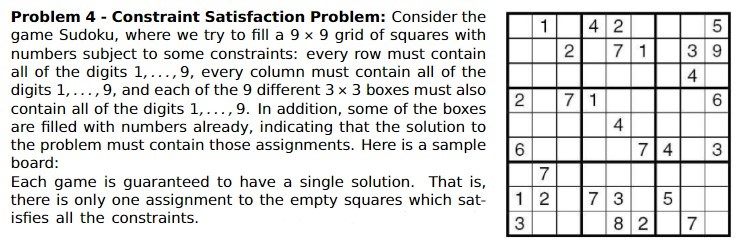
\includegraphics[width=\textwidth]{homework1/images/probdescrips/prob4.jpg}
	\caption{Sample Sudoku start state, with description of constraints and goals.}
	\label{fig:prob4}
\end{figure}

\begin{enumerate}[label=(\alph*)]

    \item \textbf{Constraint Satisfaction Problem components.}
        \begin{itemize}
            \item \textbf{Variables.} In a Sudoku problem, our variable set consists of elements representative of each small blank cell $n_{i,j}$, where $i$ represents the row of the cell and $j$ is its column. An example is shown in Figure 11. 
            \item \textbf{Domain.} For classic 9x9 Sudoku puzzles, variables can be  any value in the domain $D =$  \{1, 2, 3, 4, 5, 6, 7, 8, 9\}.
            \item \textbf{Constraints.} The constraints for any Sudoku problem are the same: any given cell cannot share the same value as any other cell in the same row, column, or within its assigned 3x3 box. There are also already cells with given values that cannot be changed. As with the variables, a partial example constraint set is shown/described in Figure 11.
        \end{itemize}

        \begin{figure}[h]
            \centering
            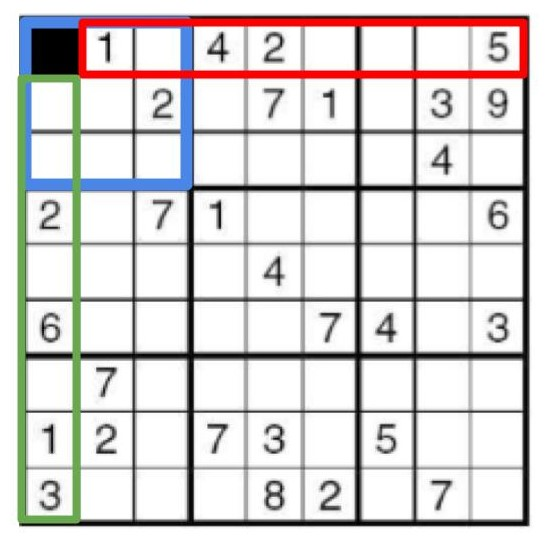
\includegraphics[scale=0.5]{homework1/images/drawndiagrams/prob4a.jpg}
	      \caption{Visualization of constraints on a given cell in Sudoku. In this figure, cell $n_{1,1}$ is shown filled in with black. The constraints on this cell are as follows: (1) this cell cannot have any of the same values as any cell in its respective column, i.e. $n_{1,1} \neq n_{i, 1}$ for any $i =$ \{2,...,9\}; (2) this cell cannot have any of the same values as any cell in its respective row, i.e. $n_{1,1} \neq n_{1,j}$ for any $j =$ \{2,...,9\}; (3) this cell cannot have any of the same values as any cell in its respective 3x3 box, i.e. $n_{1,1} \neq n_{i,j}$ for any $i$ = \{1,2,3\} and $j$ = \{1,2,3\} (excluding $(i,j) = (1,1)$, of course); (4) this cell cannot share any of the predetermined values already in its column, row, and 3x3 box, i.e. $n_{1,1} \neq$ \{1,2,3,4,5,6\}.}
	      \label{fig:prob4a}
        \end{figure}
        
    \item \textbf{Incremental formulation and backtracking search.}
        \begin{enumerate}
            \item[(i)] \textbf{Formalization.} In an incremental formulation for a Sudoku puzzle, the start state is a Sudoku grid with $M$ given values that must not be changed (given constraints). The successor function could be choosing which blank cell to fill in next and then assigning any integer between (inclusive) 1 to 9, in any particular order -- an example order of cell selection would be left to right, up to down. A goal test will check for any inconsistencies (if any constraints of the Sudoku game are violated), and return a solution when the Sudoku grid has no blank cells and no inconsistencies. A path cost would be 1 for any action.
            \item[(ii)] \textbf{Heuristic.} The minimum remaining values heuristic would work better for solving a Sudoku puzzle when using backtracking search. By filling in values that are almost obvious, if not inarguable, the rest of the grid will fill itself up rather quickly. The more cells we determine absolutely certain values for, the more constraints we put on other blank cells, making them easier to solve.
            \item[(iii)] \textbf{Size of problem.} The branching factor is the size of the domain; therefore each variable can spawn 9 children in a search tree. The maximum depth will be the number of squares that need to be filled (the total number of cells in the grid minus the total number of given solved cells in the start state), which is 81 - $M$; this is also the solution depth, since every blank cell must be explored and assigned a value. Therefore the state space for any given valid puzzle is $9^{81-M}$. 
        \end{enumerate}
    
    \item \textbf{Discerning difficulty.} The difference between ``easy" and ``hard" Sudoku problems simply lies in (1) how many constraints are put on each blank cell from the start, or more simply, how many values are given in the starting state and (2) how each new assigned value contributes to other blank cells' possible values. 
    
    When using the minimum remaining values heuristic to start on an ``easy" Sudoku problem, the domain on a starting cell is much more restrictive/easier to solve simply because it is subject to so many constraints from the already given numbers (in some cases, so constricting that the starting blank cell can only possibly have one value). In other words, in an ``easy" Sudoku problem, it is easy to gain more information from the very beginning and build on it. However, in a ``hard" Sudoku problem, each blank cell is subject to much less constraint, or constraints that are unhelpful/relatively unrelated. Starting with a minimum remaining values heuristic is difficult because even when the starting cell has a high number of constraints relative to the other cells in the puzzle, there are still \textit{several} possibilities for that starting cell, leaving little room for gaining any helpful information.

    Further, when using the maximum degree heuristic to continue to incrementally fill in values, it's easier to pick which cells to continue with in an ``easy" Sudoku puzzle than a ``hard" one, for the same reasons that a minimum remaining values heuristic is less helpful in a ``hard" puzzle than an ``easy" one. In an ``easy" Sudoku puzzle, the constraints may initially be set up in such a way that each new piece of information immediately gives way to another cell's value (or narrows its options down significantly), so it's much easier to select variables to continue to increment on. However, for a ``hard" puzzle, new information may not have much immediate impact, if at all; picking a new variable to expand on will be almost random and lead to more possible backtracking.

    \begin{algorithm}
        \caption{\texttt{Solve a Sudoku puzzle using local search.}}
        \KwIn{Sudoku puzzle to be solved, max iterations (in case of invalid puzzle)}
        \KwOut{Solution to given Sudoku puzzle (returns null if no solution)}
        // Randomly assign any value \{1, ... , 9\} to all variables (start state) \\
        possible\_solution = random\_assign(input\_start\_board) \\
        \For{$i = 0$, $i < max\_iterations$, $i{+}{+}$}{
            \If {consistent(possible\_solution)} {
                \Return {possible\_solution} \\
            }
            // Choose a variable $n_{i,j}$ that is inconsistent and reassign value randomly \\
            possible\_solution = change\_n(possible\_solution, $n_{i,j}$) \\
        }
        // No solution found -- invalid puzzle \\
        \Return{null}
    \end{algorithm}
    
    \item \textbf{Local search algorithm.} This algorithm could be quite useful for ``hard" Sudoku puzzles in comparison to a good incremental search, since we've already discussed that heuristics aren't much help for difficult puzzles; assigning values at random will most likely lead to a better solution faster than an iterative search. However, for an ``easy" Sudoku puzzle, an incremental search using a minimum remaining values heuristic would be much more beneficial than using local search since the majority of blank cells won't have many values to choose from in the first place. Random assignment in an ``easy" Sudoku would essentially be wasting time, exploring options that aren't necessary when there are already plenty of constraints to work with to gain more useful information.
    
    

\end{enumerate}


\rule{\linewidth}{0.4pt}
\vspace{.2cm}

%%%%%%%%%%%%%%%%%%%%%%%%%
%%%%%%%%%%%%%%% Problem 5
%%%%%%%%%%%%%%%%%%%%%%%%%
\textbf{Problem 5 - Logic-based Reasoning (5 points):}

\vspace{.5cm}

\noindent \textit{For Superman to be defeated, it has to be that he is facing an opponent alone and his opponent is carrying Kryptonite. Acquiring Kryptonite, however, means that Batman has to coordinate with Lex Luthor and acquire it from him. If, however, Batman coordinates with Lex Luthor, this upsets Wonder Woman, who will intervene and fight on the side of Superman.}

\begin{enumerate}[label=(\alph*)]

    \item \textbf{Converting to symbols.} In order to convert the above statements to propositional logic, we must first assign propositions to symbols (in this case, capital letters). For this example:
    \begin{itemize}
        \item $A$: Superman can be defeated.
        \item $B$: Superman is alone.
        \item $C$: Batman has Kryptonite.
        \item $D$: Batman went to Lex Luthor.
        \item $E$: Wonder Woman fights with Superman.
    \end{itemize}
    
    Now, we can directly translate the paragraph into a knowledge base. 

    \begin{itemize}
        \item $A \iff (B \land C)$: For Superman to be defeated, it has to be that he is facing an opponent alone and his opponent is carrying Kryptonite.
        \item $C \implies D$: Acquiring Kryptonite, however, means that Batman has to coordinate with Lex Luthor and acquire it from him.
        \item $D \implies E$: If, however, Batman coordinates with Lex Luthor, this upsets Wonder Woman, who will intervene and fight on the side of Superman.
    \end{itemize}
    ** Despite not being explicitly stated, we can infer that if Wonder Woman fights with Superman ($E$), then Superman is not alone ($\neg B$). This can be added to our knowledge base, written in propositional logic as $E \implies \neg B$.

    \item \textbf{Simplifying/expanding.} Now let's translate our knowledge into 3-CNF statements:

        \begin{itemize}{}
            \item $A \iff (B \land C)$ can be expanded to $(A \implies (B \land C)) \land ((B \land C) \implies A)$ using bi-conditional elimination. 
        
            This can then be rewritten as $(\neg A \lor (B \land C)) \land ((\neg B \lor \neg C) \lor A)$ using implication elimination and some DeMorgan's Law. 
        
            To fully convert the statement into 3-CNF form, we can distribute the $\lor$ in the first clause, giving us $(\neg A \lor B) \land (\neg A \lor C) \land (\neg B \lor \neg C \lor A)$.
        
            \item $C \implies D$ can be rewritten as $\neg C \lor D$ using implication elimination.
            \item $D \implies E$ can be rewritten as $\neg D \lor E$ using implication elimination.
            \item $E \implies \neg B$ can be rewritten as $\neg E \lor \neg B$ using implication elimination.
        \end{itemize}
    By combining all of our established rules, we obtain the knowledge base:
    
    $(\neg A \lor B) \land (\neg A \lor C) \land (\neg B \lor \neg C \lor A) \land (\neg C \lor D) \land (\neg D \lor E) \land (\neg E \lor \neg B)$

    \item \textbf{Proof.} We want to prove that Batman cannot defeat Superman ($\neg A$). Therefore, we will show a proof by contradiction, only using the resolution inference rule to simplify, by showing $KB  \land A$ (the knowledge base and the negation of our hypothesis) is implausible.
    \begin{enumerate}
        \item [(1)] $(\neg A \lor B) \land (\neg A \lor C) \land (\neg B \lor \neg C \lor A) \land (\neg C \lor D) \land (\neg D \lor E) \land (\neg E \lor \neg B) \land A$
        \item [(2)] $B \land C \land (\neg B \lor \neg C \lor A) \land (\neg C \lor D) \land (\neg D \lor E) \land (\neg E \lor \neg B) \land A$
        \item [(3)] $B \land C \land (\neg B \lor \neg C \lor A) \land (\neg C \lor E) \land (\neg E \lor \neg B) \land A$
        \item [(4)] $B \land C \land (\neg B \lor \neg C \lor A) \land (\neg C \lor \neg B) \land A$
        \item [(5)] $B \land C \land (\neg B \lor \neg C \lor A) \land \neg B \land A$
    \end{enumerate}
    At this point, we have reached a contradiction: when assuming $A$ in conjunction with our knowledge base, this leads to $B \land \neg B$ being true, which is implausible. This means $\neg A$ must be true; we have shown that with the given conditions, it is impossible for Batman to defeat Superman.
\end{enumerate}

\end{document}